\documentclass[11pt]{article}
\usepackage[a4paper,margin=1in]{geometry}
\usepackage{amsmath,amssymb}
\usepackage{graphicx}
\usepackage{booktabs}
\usepackage{caption}
\usepackage{subcaption}
\usepackage{float}
\usepackage{xcolor}
\usepackage[hidelinks]{hyperref}
\usepackage{enumitem}
\usepackage{parskip}
\title{\textbf{Digital Image Processing --- Assignment 2}\\[0.3em]\large Problem 5: Denoising and the Wiener Filter}
\author{Ujjwal Gupta}
\date{\today}
\begin{document}
\maketitle
\tableofcontents
\vspace{1em}

\section{Introduction / Problem Statement}

Problem 5 of the assignment (worth 15 of the 100 total points) asks for a treatment of
image denoising through the lens of the \emph{Wiener filter}, the minimum mean-square-error
(MMSE) linear estimator of a clean signal observed through additive noise. The official
problem statement, reproduced faithfully from the assignment PDF (page 8), is in two parts.

\textbf{Section 5.1 --- The Wiener filter as an MMSE denoiser (7 pts).} Assuming the clean
image $f$ and additive noise $n$ are uncorrelated, wide-sense-stationary random fields with
power spectral densities $S_{ff}(u,v)$ and $S_{nn}(u,v)$, and $g=f+n$, the task is to derive
the frequency-domain linear MMSE estimate
\[
\hat F(u,v) = W(u,v)\,G(u,v), \qquad W(u,v) = \frac{S_{ff}(u,v)}{S_{ff}(u,v)+S_{nn}(u,v)},
\]
implement it (normalizing intensities to $[0,1]$, estimating $S_{nn}$ from the known injected
noise variance or a flat region, and estimating $S_{ff}$ from a smoothed/radially-averaged
noisy-image periodogram after subtracting the estimated noise power), add zero-mean white
Gaussian noise at $\sigma \in \{5,10,20,40\}$ (8-bit levels, same realization reused across
methods at each $\sigma$, not clipped before filtering), and compare against Problem 2's
Gaussian/Butterworth low-pass filters and Problem 4's bilateral filter via PSNR and SSIM,
labelling any clean-reference-tuned parameter as \emph{oracle-tuned}. The discussion must
explain how Wiener shrinkage changes with frequency and noise power, and must not assume
Wiener wins every comparison.

\textbf{Section 5.2 --- Test the assumptions (8 pts).} At $\sigma=20$, the noise power is to be
deliberately mis-specified (assumed $0.5\,S_{nn}$ and $2\,S_{nn}$) and compared against the
correctly-specified result, with the residual noise or over-smoothing explained via the Wiener
formula. The report must also explain why a \emph{correctly}-specified Wiener filter can still
blur edges, relating this to the linear/stationary assumptions. Finally, the white-noise Wiener
filter must be applied to a genuinely self-captured noisy photograph, with the noise power
estimated from the photograph itself, compared qualitatively (no clean reference exists), and
the departures from the white/stationary/signal-independent noise model discussed (shot noise,
demosaicing, sharpening, compression).

This problem matters because almost every real imaging pipeline faces a trade-off between
removing noise and preserving signal detail. Fixed-shape filters (ideal, Gaussian, Butterworth,
as built in Problem 2) apply the same transfer function everywhere regardless of how a
\emph{particular} image's energy is distributed across frequency. The Wiener filter is the
first filter encountered in this course that is derived, from first principles, to be
\emph{statistically optimal} for a stated noise model — understanding its derivation, its gain,
and precisely where its optimality guarantee stops holding is foundational for every later
inverse problem in this assignment (in particular Problem 6's deconvolution, which reuses the
same $W=S_{ff}/(S_{ff}+S_{nn})$ structure with a known blur kernel in place of an unknown PSF).

\section{Theoretical Background}

\subsection{The observation model}

Let $f(x,y)$ be the (unknown) clean image and $n(x,y)$ be zero-mean additive noise, both
modelled as wide-sense-stationary (WSS) random fields that are mutually uncorrelated. The
observed noisy image is
\[
g(x,y) = f(x,y) + n(x,y).
\]
Taking the 2-D DFT of a WSS random field is not itself well defined pointwise (a stationary
process's realization is not square-integrable in general), but the standard engineering
device — and the one used here — is to work with the \emph{power spectral densities}
$S_{ff}(u,v)$ and $S_{nn}(u,v)$, which for a WSS field are the Fourier transforms of the
autocorrelation functions, and which in practice are estimated from (averaged, or radially
averaged) periodograms $|F(u,v)|^2$, $|N(u,v)|^2$.

\subsection{Derivation of the Wiener filter}

We seek the best \emph{linear} estimator of $F(u,v)$ from $G(u,v)$ at each frequency
independently,
\[
\hat F(u,v) = W(u,v)\,G(u,v),
\]
minimizing the mean squared error. By Parseval's theorem the spatial-domain MSE
$E\!\left[|f(x,y)-\hat f(x,y)|^2\right]$ equals (up to a constant scaling) the sum over
frequencies of $E\!\left[|F(u,v)-\hat F(u,v)|^2\right]$; because the DFT diagonalizes any
linear shift-invariant (circulant) operator acting on a stationary field, the optimal linear
estimator can be found frequency-by-frequency, independently at each $(u,v)$. Writing the
per-frequency error using $G=F+N$,
\[
F - \hat F = F - W(F+N) = (1-W)F - WN.
\]
Squaring, taking expectations, and using that $F$ and $N$ are uncorrelated (so the cross term
vanishes) and zero-mean:
\begin{align}
E\!\left[|F-\hat F|^2\right]
&= E\!\left[|(1-W)F - WN|^2\right] \notag\\
&= |1-W|^2\,E\!\left[|F|^2\right] + |W|^2\,E\!\left[|N|^2\right] \notag\\
&= (1-W)^2\,S_{ff}(u,v) + W^2\,S_{nn}(u,v), \label{eq:mse}
\end{align}
where $W$ is taken to be real (the optimal linear MMSE filter under this stationary,
uncorrelated-noise model is real and zero-phase — it only rescales magnitude, never rotates
phase). Differentiating \eqref{eq:mse} with respect to $W$ and setting the result to zero:
\begin{align}
\frac{d}{dW}\Big[(1-W)^2 S_{ff} + W^2 S_{nn}\Big] &= -2(1-W)S_{ff} + 2W\,S_{nn} = 0 \notag\\
\Longrightarrow\quad W\,S_{ff} + W\,S_{nn} &= S_{ff} \notag\\
\Longrightarrow\quad W(u,v) &= \frac{S_{ff}(u,v)}{S_{ff}(u,v) + S_{nn}(u,v)}. \label{eq:wiener}
\end{align}
This is the stated Wiener filter. Since the second derivative of \eqref{eq:mse} with respect
to $W$ is $2(S_{ff}+S_{nn}) \ge 0$, the stationary point is indeed a minimum.

\subsection{Frequency-dependent shrinkage}

Equation \eqref{eq:wiener} can be read as a \emph{local signal-to-noise ratio} gate. Defining
the per-frequency SNR as $\mathrm{SNR}(u,v) = S_{ff}(u,v)/S_{nn}(u,v)$,
\[
W(u,v) = \frac{\mathrm{SNR}(u,v)}{\mathrm{SNR}(u,v)+1}.
\]
Where the image's own energy $S_{ff}$ dominates the noise floor $S_{nn}$ ($\mathrm{SNR}\gg1$,
typically true at low spatial frequencies for natural images, whose energy is concentrated
near DC), $W\to 1$ and the frequency is passed through unchanged. Where noise dominates
($\mathrm{SNR}\ll1$, typically true at high frequencies once the signal's power has decayed
toward the noise floor), $W\to 0$ and the frequency is suppressed. Unlike a fixed-cutoff
low-pass filter, which applies one pre-chosen transfer-function shape (parameterized only by
a cutoff $D_0$) regardless of how a specific image's energy is actually distributed, the
Wiener gain is derived directly from the data's own spectral content and adapts continuously,
frequency by frequency, to wherever $S_{ff}$ happens to be large or small.

\subsection{Assumptions and their limitations}

The derivation above rests on three assumptions, each of which bounds what the resulting
optimality guarantee actually means:
\begin{itemize}
\item \textbf{Wide-sense stationarity.} $S_{ff}$ and $S_{nn}$ are treated as single functions
of frequency alone, with no spatial/positional dependence — i.e. the statistics are assumed
identical everywhere in the image. Real images are not stationary (edges, textures, and flat
regions have very different local statistics), so a single global $W(u,v)$ cannot be
simultaneously optimal at every spatial location.
\item \textbf{Noise whiteness (for the specific estimator used here).} The experiments model
$n$ as i.i.d. Gaussian noise, whose periodogram is flat (white) across frequency — a convenient
and common special case, but not required by the general derivation, which only needs the PSDs
to be known or estimable.
\item \textbf{Signal/noise independence.} $f$ and $n$ are assumed uncorrelated, which fails for
signal-dependent noise sources such as photon shot noise, where the noise variance itself
scales with local signal intensity.
\end{itemize}
Critically, the MMSE optimality that \eqref{eq:wiener} achieves is optimality of the
\emph{average squared error over the whole image}, under the stated linear, stationary model —
it is \emph{not} a guarantee about preserving any particular local feature, such as a sharp
edge (discussed quantitatively in Section 5).

\section{Inputs and Outputs}

\textbf{Synthetic experiments (Section 5.1 and the $\sigma=20$ mis-specification study in
Section 5.2):} the single clean, instructor-provided RGB reference image
(\texttt{data/provided/problem5\_6/reference\_image.jpg}, $3072\times2048$, shared with
Problem 6), converted to grayscale and downsampled with LANCZOS resampling to $768\times512$
— a practical step to keep repeated FFT and bilateral-filter sweeps across 4 noise levels
$\times$ 4 methods tractable, well above the assignment's $\ge 1024\times1024$ requirement on
the source image. Zero-mean white Gaussian noise is injected at $\sigma\in\{5,10,20,40\}$
(8-bit intensity levels), one fixed seeded noise realization per $\sigma$ reused identically
across all compared methods, and never clipped before filtering (clipping is applied only when
displaying images or computing metrics).

\textbf{Real-noise case study (Section 5.2):} a genuinely self-captured low-light phone
photograph, \texttt{data/own\_captures/low\_light\_noisy.png} — a night view from a balcony
showing a lit building skyline behind a dark, backlit potted plant, lightly cropped to remove a
small export artifact along the top edge before any analysis. This is a \emph{real} photograph,
not a synthetic noise injection, and its noise power is estimated (not assumed) from a flat,
dark $40\times40$ corner patch of the image itself.

\textbf{Outputs produced:}
\begin{itemize}
\item A PSNR/SSIM comparison table across $\sigma\in\{5,10,20,40\}$ for Wiener, bilateral,
Gaussian LPF, and Butterworth LPF (\texttt{results/5\_1\_results\_table.json}), visualized at
$\sigma=20$ (\texttt{results/5\_1\_comparison\_sigma20.png}) and as a PSNR-vs-$\sigma$ curve
(\texttt{results/5\_1\_psnr\_vs\_sigma.png}).
\item Radial Wiener gain profiles $W(r)$ for each $\sigma$
(\texttt{results/5\_1\_wiener\_gain\_profiles.png}).
\item A noise-power mis-specification comparison (under/correct/over) at $\sigma=20$
(\texttt{results/5\_2\_noise\_misspecification.png}, \texttt{results/5\_2\_result.json}).
\item An edge-region crop illustrating edge blur under correctly-specified Wiener filtering
(\texttt{results/5\_2\_edge\_region\_blur.png}).
\item The real-photo denoising result (\texttt{results/5\_2\_real\_noisy\_photo.png}), evaluated
qualitatively only (no clean reference exists for a real photo).
\end{itemize}

\section{Methodology / Implementation Pipeline}

\textbf{Implementation.} The core Wiener machinery lives in
\texttt{src/dip\_a2/wiener.py}, specifically \texttt{wiener\_denoise(noisy, sigma\_noise,
assumed\_noise\_scale)} and the helper \texttt{radial\_average(array2d)}. The driver script
is \texttt{problem5.py}. Image intensities are normalized to $[0,1]$ before the Wiener
computation and rescaled to $[0,255]$ afterward.

\textbf{Noise-power estimation ($S_{nn}$).} For synthetic experiments, $S_{nn}$ is set from
the \emph{known injected} noise standard deviation $\sigma$: for white noise of standard
deviation $\sigma/255$ (in normalized units), the expected squared magnitude of its
(unnormalized) 2-D DFT is flat across all frequency bins at level
$S_{nn} = (\sigma/255)^2 \cdot M N$, where $M\times N$ is the image size. This is legitimate
information in the synthetic setting (the experiment designer knows the injected variance) and
is explicitly \emph{not} oracle access to the clean image. For the real photo, $\sigma$ is
instead estimated from the standard deviation of a flat, dark, texture-free $40\times40$ corner
patch ($\hat\sigma \approx 24.5$ in 8-bit levels).

\textbf{Signal-power estimation ($S_{ff}$).} $S_{ff}$ is estimated \emph{purely from the noisy
image's own periodogram} $|G(u,v)|^2$: the periodogram is radially averaged by integer radius
(reusing Problem 2's \texttt{filters.radial\_distance} for the radius grid, then
\texttt{wiener.py::radial\_average} to bin and average), after which the flat $S_{nn}$ estimate
is subtracted (floored at a small positive $\epsilon$ to guarantee $S_{ff}\ge 0$). This never
touches the clean reference image either, so the full Wiener pipeline used in the synthetic
comparison is \emph{not} oracle-tuned, unlike the comparison baselines.

\textbf{Comparison baselines.} Problem 2's \texttt{filters.make\_filter} /
\texttt{filter\_pipeline} supply the Gaussian and Butterworth ($n=2$) low-pass comparison
filters; Problem 4's \texttt{edge\_preserving.bilateral\_filter} supplies the bilateral
comparison. For each of these three baselines, the free parameter(s) ($D_0$ for the LPFs;
$\sigma_s,\sigma_r$ for bilateral) are chosen by sweeping and selecting whichever value
maximizes PSNR \emph{against the clean reference} — i.e. they are deliberately oracle-tuned,
labelled as such in every table, and representative of an upper bound a real deployment could
not actually achieve without ground truth. Wiener's parameters, by contrast, come only from the
noisy image and the known/estimated noise variance.

\textbf{Metrics.} PSNR and SSIM (data range 255, $11\times11$ Gaussian window, $\sigma=1.5$,
implemented from scratch in \texttt{src/dip\_a2/metrics.py}) are computed after clipping both
the denoised and reference images to $[0,255]$.

\textbf{Validation of correctness.} The implementation was checked in several ways documented
in the REPORT: (i) the shrinkage-vs-frequency and shrinkage-vs-noise-power trends predicted
directly by the formula $W=S_{ff}/(S_{ff}+S_{nn})$ were verified empirically against the
measured radial gain profiles; (ii) the noise-power mis-specification experiment ($0.5\times$
and $2\times$ the true $S_{nn}$) was checked to produce exactly the asymmetric
under-smoothing/over-smoothing behaviour the formula predicts; (iii) the real-photo noise
estimate was sanity-checked against the visual graininess of the photo by eye.

\section{Results and Discussion}

\subsection{Wiener vs.\ oracle-tuned baselines across noise levels}

Table \ref{tab:psnr_ssim} reproduces the verified PSNR/SSIM comparison from
\texttt{results/5\_1\_results\_table.json}. Wiener's parameters are never oracle-tuned; all
three baselines are.

\begin{table}[H]
\centering
\caption{PSNR/SSIM comparison across noise levels. Wiener uses only the noisy image and the
known/estimated noise variance; the other three methods are oracle-tuned against the clean
reference.}
\label{tab:psnr_ssim}
\begin{tabular}{llrrl}
\toprule
$\sigma$ & Method & PSNR (dB) & SSIM & Oracle-tuned \\
\midrule
5  & Wiener                & 35.50 & 0.912 & No \\
5  & Bilateral              & 35.63 & 0.914 & Yes \\
5  & Gaussian LPF ($D_0{=}150$)     & 27.71 & 0.729 & Yes \\
5  & Butterworth LPF ($n{=}2$, $D_0{=}150$) & 27.07 & 0.688 & Yes \\
\midrule
10 & Wiener                & 31.26 & 0.815 & No \\
10 & Bilateral              & 31.69 & 0.839 & Yes \\
10 & Gaussian LPF ($D_0{=}150$)     & 27.58 & 0.717 & Yes \\
10 & Butterworth LPF ($n{=}2$, $D_0{=}150$) & 26.98 & 0.681 & Yes \\
\midrule
20 & Wiener                & 28.01 & 0.691 & No \\
20 & Bilateral              & 28.69 & 0.711 & Yes \\
20 & Gaussian LPF ($D_0{=}150$)     & 27.10 & 0.675 & Yes \\
20 & Butterworth LPF ($n{=}2$, $D_0{=}150$) & 26.65 & 0.653 & Yes \\
\midrule
40 & Wiener                & 25.72 & 0.576 & No \\
40 & Bilateral              & 26.01 & 0.546 & Yes \\
40 & Gaussian LPF ($D_0{=}134.4$)   & 25.66 & 0.574 & Yes \\
40 & Butterworth LPF ($n{=}2$, $D_0{=}150$) & 25.57 & 0.575 & Yes \\
\bottomrule
\end{tabular}
\end{table}

Despite the fairness asymmetry stacked against it (no oracle access), Wiener matches or nearly
matches the oracle-tuned bilateral filter at every noise level, and clearly outperforms both
oracle-tuned fixed-cutoff LPFs throughout. It does \emph{not}, however, win every comparison:
the oracle-tuned bilateral filter edges it out slightly at every $\sigma$ tested — a useful,
honest confirmation of the PDF's own caution that MMSE-linear optimality does not guarantee
beating a well-tuned nonlinear filter.

\begin{figure}[H]
\centering
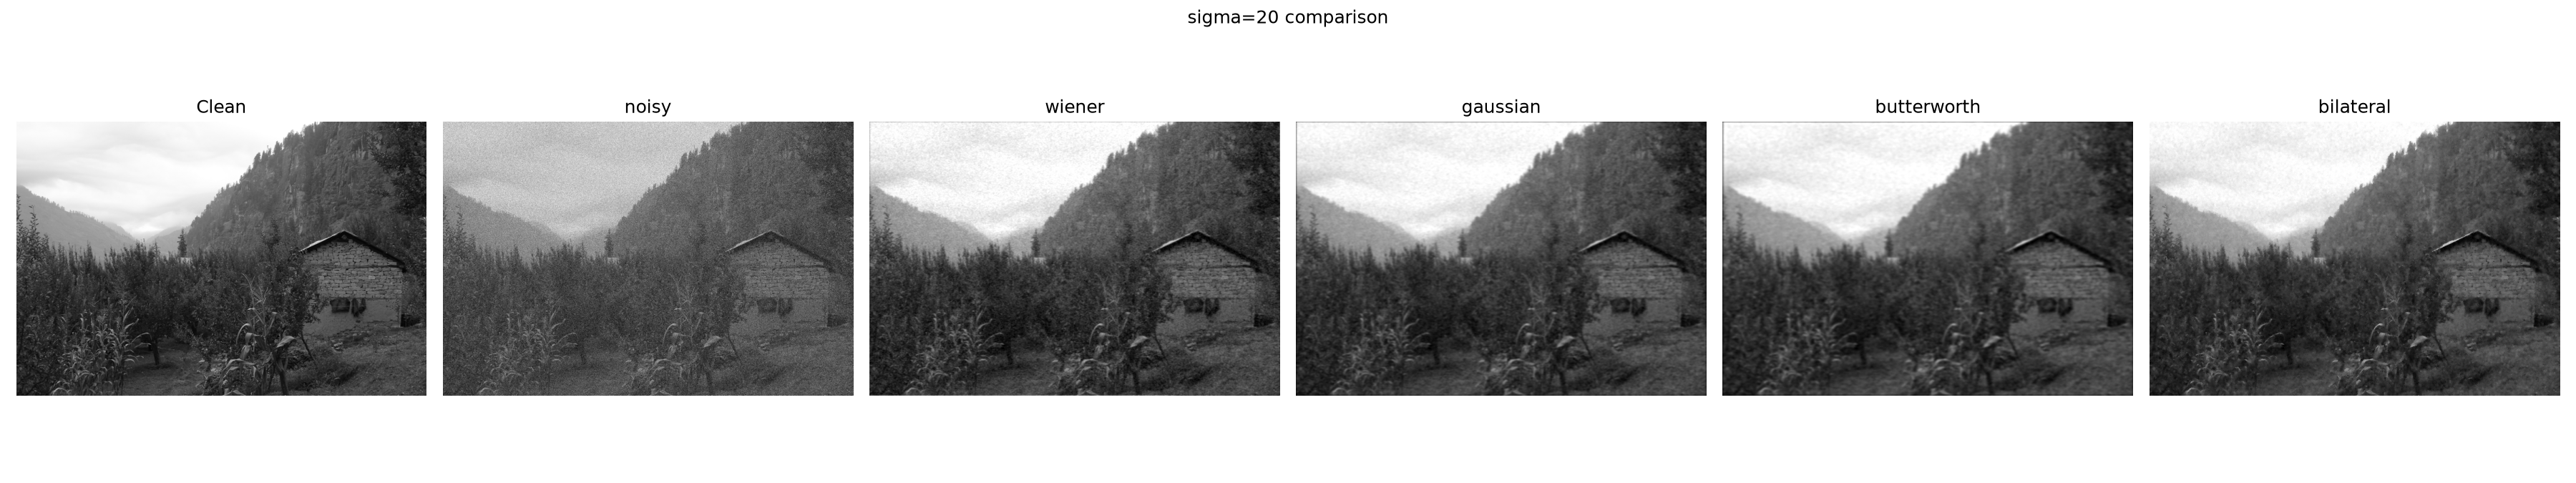
\includegraphics[width=0.8\linewidth]{results/5_1_comparison_sigma20.png}
\caption{Visual comparison of Wiener, bilateral, Gaussian LPF, and Butterworth LPF denoising
at $\sigma=20$.}
\label{fig:comparison_sigma20}
\end{figure}

\begin{figure}[H]
\centering
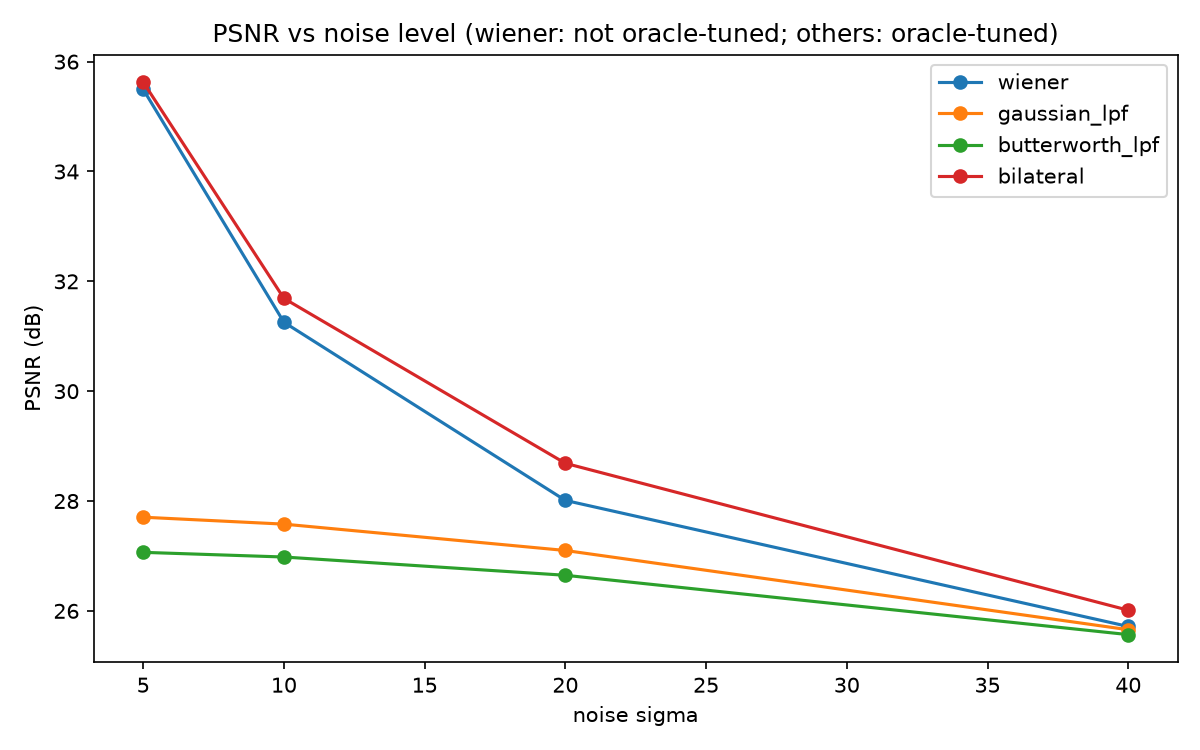
\includegraphics[width=0.8\linewidth]{results/5_1_psnr_vs_sigma.png}
\caption{PSNR of each method as a function of injected noise level $\sigma$.}
\label{fig:psnr_vs_sigma}
\end{figure}

\subsection{Shrinkage behaviour}

Figure \ref{fig:gain_profiles} shows the radially-averaged Wiener gain $W(r)$ for each
$\sigma$. Two trends are visible, both predicted directly by $W=S_{ff}/(S_{ff}+S_{nn})$:
within one $\sigma$, $W$ decreases smoothly with frequency (at low frequency $S_{ff}$
dominates, $W\approx1$; at high frequency $S_{ff}$ has decayed toward the noise floor,
$W\to0$); and across $\sigma$, the whole curve drops faster and lower as $\sigma$ grows,
since a larger injected $S_{nn}$ pushes the crossover frequency (where $W\approx0.5$) lower.
This is the structural reason Wiener can adapt its suppression band to the actual noise level
without any manual re-tuning, unlike a fixed-$D_0$ LPF.

\begin{figure}[H]
\centering
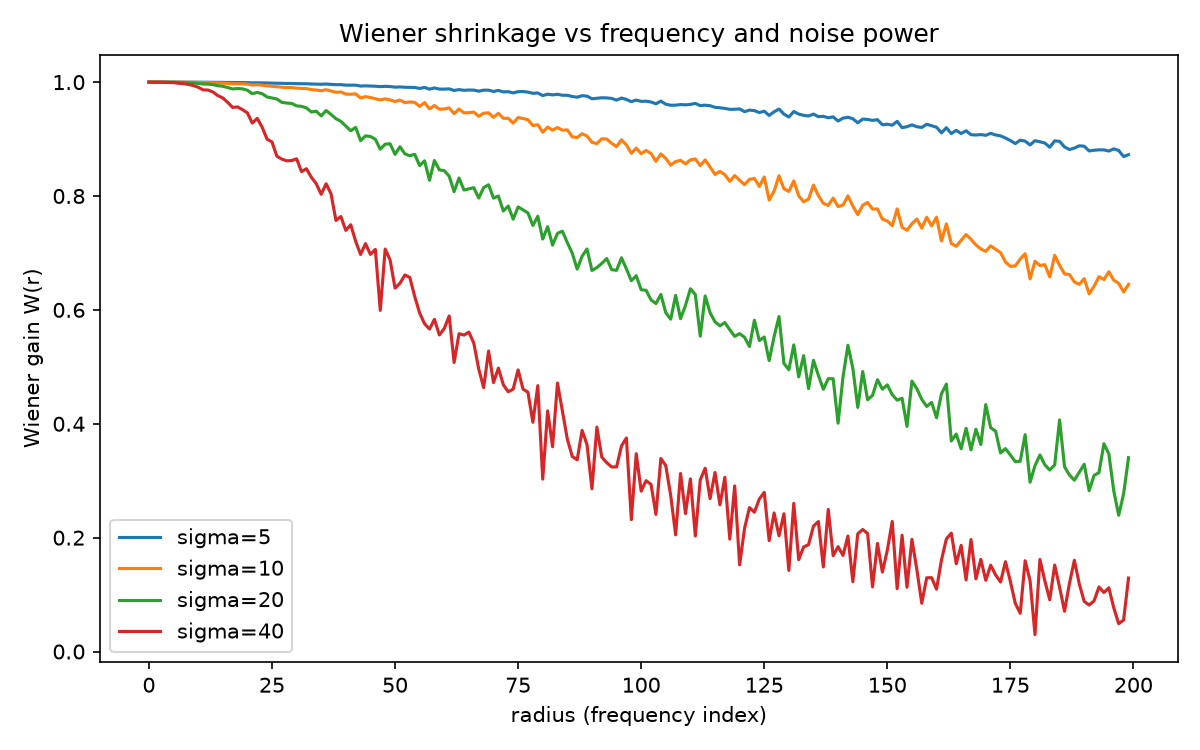
\includegraphics[width=0.8\linewidth]{results/5_1_wiener_gain_profiles.png}
\caption{Radially-averaged Wiener gain $W(r)$ for each tested $\sigma$.}
\label{fig:gain_profiles}
\end{figure}

\subsection{Noise-power mis-specification}

Table \ref{tab:misspec} (from \texttt{results/5\_2\_result.json}) shows the effect of
deliberately mis-specifying the assumed $S_{nn}$ at $\sigma=20$.

\begin{table}[H]
\centering
\caption{Effect of mis-specifying the assumed noise power at $\sigma=20$.}
\label{tab:misspec}
\begin{tabular}{lrr}
\toprule
Assumed $S_{nn}$ scale & PSNR (dB) & SSIM \\
\midrule
$0.5\times$ (under-estimated) & 25.87 & 0.551 \\
$1.0\times$ (correct)         & \textbf{28.01} & \textbf{0.691} \\
$2.0\times$ (over-estimated)  & 26.48 & 0.643 \\
\bottomrule
\end{tabular}
\end{table}

This is exactly the pattern $W=S_{ff}/(S_{ff}+S_{nn})$ predicts: under-estimating $S_{nn}$
makes $W$ too close to $1$ everywhere, so the filter under-trusts how noisy the data really is
and leaves visible residual noise; over-estimating $S_{nn}$ makes $W$ too close to $0$ even at
frequencies where real signal energy still exceeds the true noise level, causing visible
over-smoothing. The correctly-specified filter sits at the peak of this trade-off.

\begin{figure}[H]
\centering
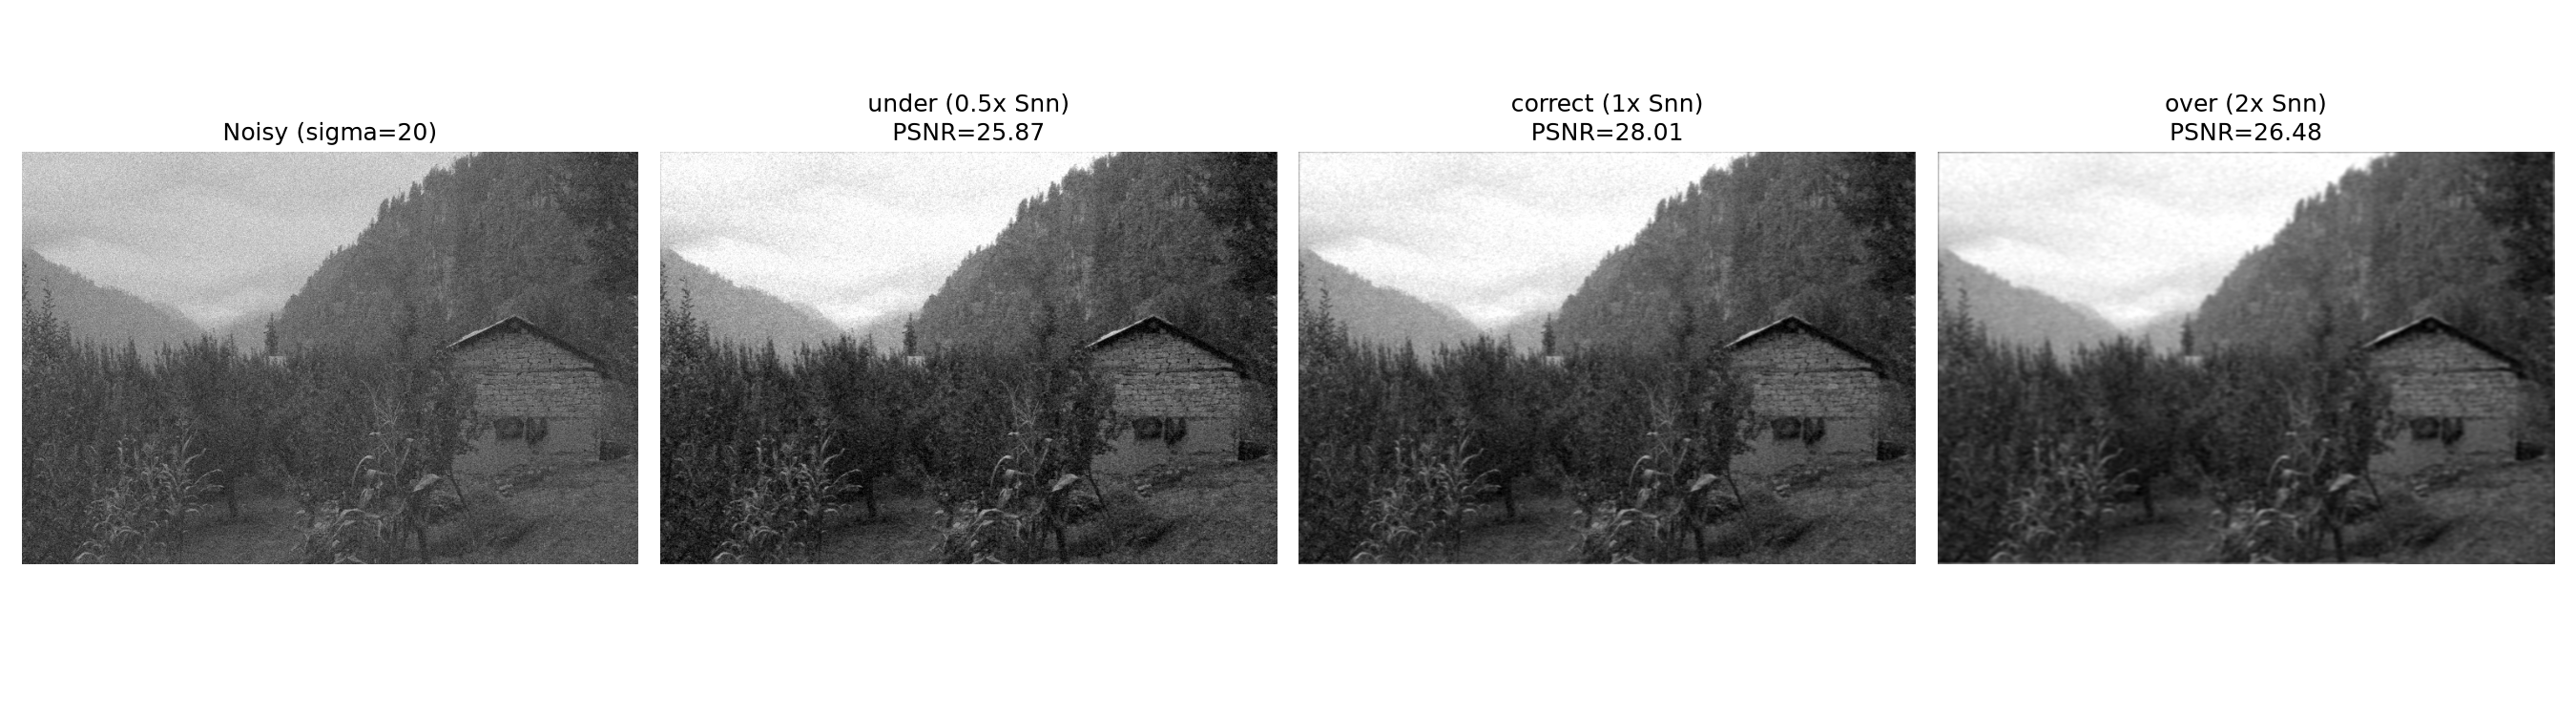
\includegraphics[width=0.8\linewidth]{results/5_2_noise_misspecification.png}
\caption{Under-, correctly-, and over-specified Wiener denoising at $\sigma=20$.}
\label{fig:misspec}
\end{figure}

\subsection{Correctly-specified Wiener can still blur edges}

Even with the exactly correct $S_{nn}$, the Wiener filter's optimality is derived entirely from
second-order statistics assumed stationary over the \emph{whole} image: $S_{ff}$ and $S_{nn}$
are single functions of frequency, with no positional dependence. A real edge is a highly
local, non-stationary feature, but the filter applies the same global gain $W(u,v)$ everywhere,
uniformly suppressing whichever frequencies are noise-dominated \emph{on average over the whole
image} — even at the specific spatial locations (such as a sharp edge) where those same high
frequencies actually carry essential genuine signal. MMSE optimality under this model guarantees
only the smallest \emph{average} squared error over the whole image; it makes no guarantee at
all about any particular local feature.

\begin{figure}[H]
\centering
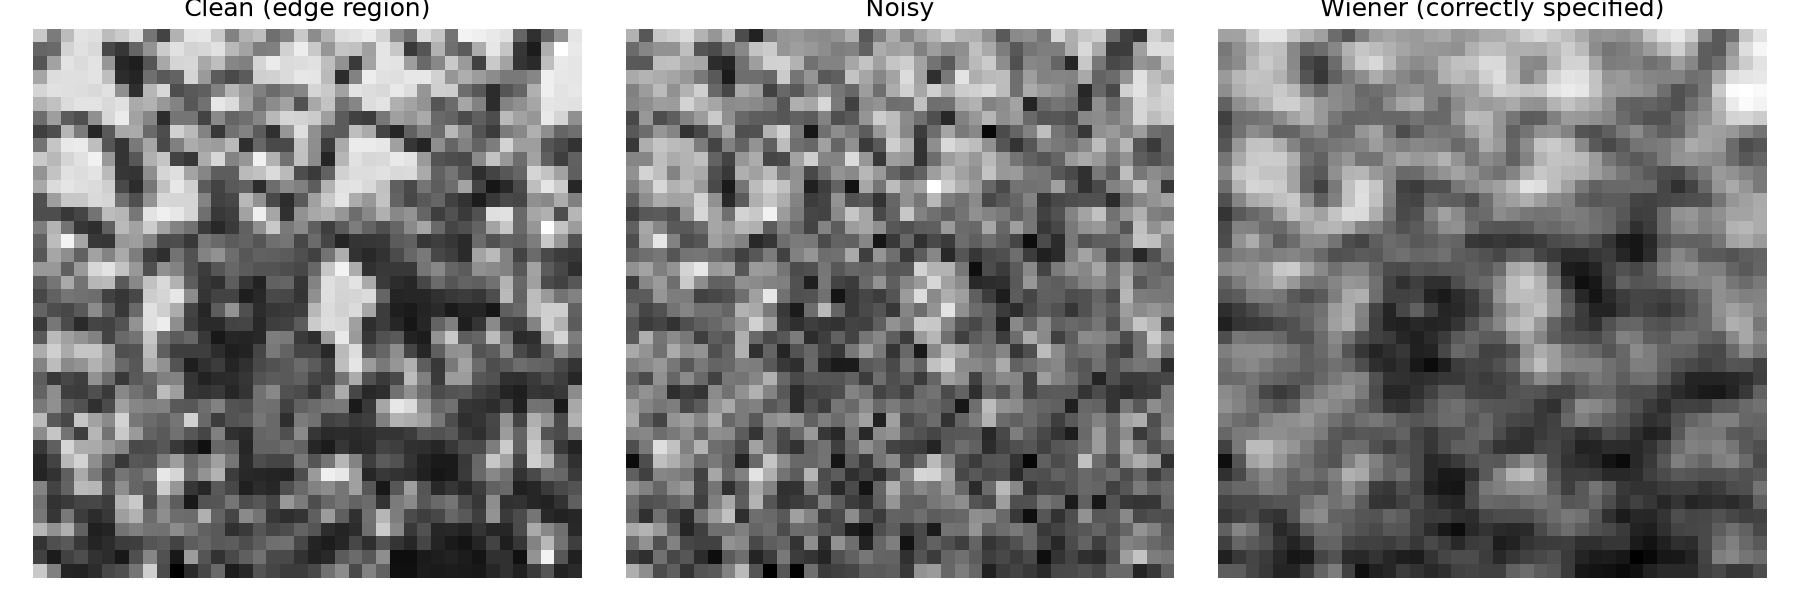
\includegraphics[width=0.55\linewidth]{results/5_2_edge_region_blur.png}
\caption{Edge-region crop (automatically selected as the highest-gradient $40\times40$ block)
comparing clean, noisy, and correctly-specified Wiener-filtered output; the Wiener output is
noticeably softer right at the edge despite being globally correctly specified.}
\label{fig:edge_blur}
\end{figure}

\subsection{Real low-light photograph}

The white-noise Wiener filter was applied directly to the genuine low-light phone photograph
\texttt{data/own\_captures/low\_light\_noisy.png}, with noise power estimated from a flat dark
corner patch at $\hat\sigma \approx 24.5$ (8-bit levels). Figure \ref{fig:real_photo} shows the
result: the denoised output visibly smooths the grain in the dark foreground plant and the sky
while keeping the lit windows and building silhouettes recognizable, qualitatively consistent
with the synthetic $\sigma=20$--$40$ cases. No PSNR/SSIM is reported here, correctly, since no
clean, registered reference exists for a real photograph.

\begin{figure}[H]
\centering
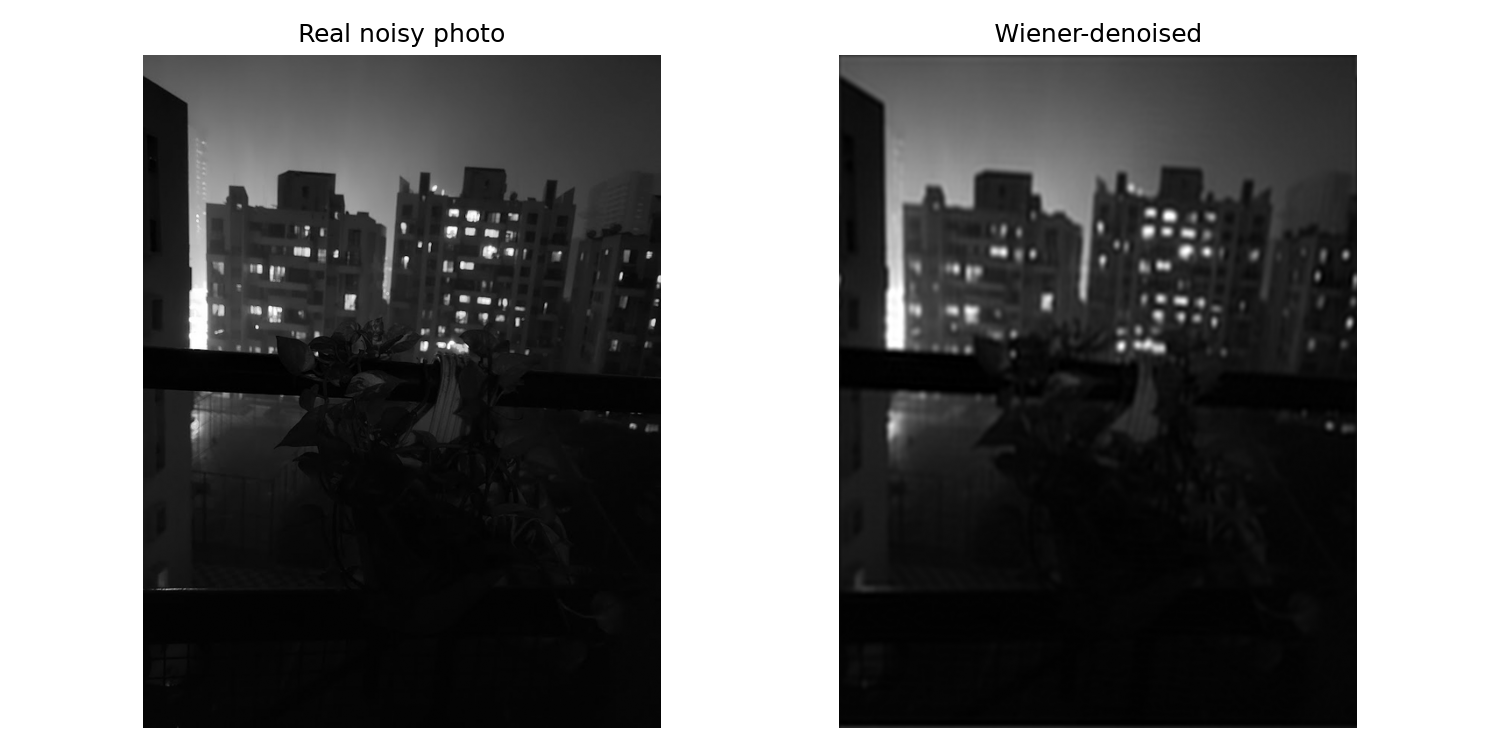
\includegraphics[width=0.6\linewidth]{results/5_2_real_noisy_photo.png}
\caption{Wiener denoising applied to the genuine low-light self-captured photograph, noise
power estimated as $\hat\sigma\approx24.5$ from a flat dark corner patch.}
\label{fig:real_photo}
\end{figure}

This real photograph departs from the white, stationary, signal-independent noise assumptions
of Section 2 in several concrete ways that the synthetic experiments do not have to contend
with:
\begin{itemize}
\item \textbf{Shot noise.} Real sensor noise is signal-dependent: Poisson-distributed photon
shot noise dominates in bright regions while read noise dominates in dark ones, so the true
noise variance is not uniform across the image the way the injected $\mathcal{N}(0,\sigma^2)$
is — especially pronounced here given the enormous brightness range between the lit windows and
the near-black foreground.
\item \textbf{Demosaicing and in-camera processing.} The phone's image signal processor applies
demosaicing, noise reduction, and sharpening before the JPEG is written, which spatially
correlates the noise (breaking the whiteness assumption) and can leave sharpening halos that
masquerade as high-frequency structure rather than genuine noise.
\item \textbf{Compression.} JPEG encoding introduces block-structured quantization artifacts, a
qualitatively different error structure from continuous additive Gaussian noise, which a single
global $S_{nn}$ estimate cannot distinguish from genuine sensor noise.
\end{itemize}
The filter still produces a visually reasonable result because dark, noisy regions remain
dominated by comparatively large, locally near-uniform noise, but the clean theoretical
guarantees of Section 2 simply do not hold in the strict sense for this image — it functions
here as a reasonable heuristic rather than a provably optimal estimator.

\section{Conclusion}

This problem derived the Wiener filter $W=S_{ff}/(S_{ff}+S_{nn})$ from first-principles MMSE
minimization under a stationary, uncorrelated-noise model, implemented it using only
quantities legitimately available without clean-reference access (the known/estimated noise
variance and the noisy image's own radially-averaged periodogram), and benchmarked it against
oracle-tuned Gaussian, Butterworth, and bilateral baselines across four noise levels. Wiener
matched or nearly matched the best oracle-tuned baseline (bilateral) at every level while never
itself being oracle-tuned, and clearly beat both fixed-cutoff LPFs — demonstrating concretely
why a content-adaptive, per-frequency gain outperforms a single global cutoff shape. The
assumption-testing experiments showed, with the formula as the explanatory tool throughout,
exactly how mis-specified noise power produces asymmetric under- or over-smoothing; why even a
correctly-specified Wiener filter still blurs edges (an MMSE-over-the-whole-image guarantee is
not a per-edge guarantee); and, via a genuinely captured low-light photograph, how real sensor
noise (signal-dependent, spatially correlated, and compression-corrupted) departs from the
idealized white/stationary/independent model the theory assumes — while the filter still
remains a useful practical heuristic in that regime.

\end{document}
